% ---
% title: LaTeX 写作示例
% date: 2026-09-20
% tag: Example
% excerpt: 本站 LaTeX 模式的完整示例：章节与交叉引用、公式、复杂表格、插图与子图、引用与参考文献、代码等日常写作场景，可直接复制作为模板。
% ---
\definecolor{oursbg}{HTML}{F6E7DE}
\newcommand{\E}{\mathbb{E}}
\newcommand{\R}{\mathbb{R}}
\newtheorem{hyp}{假设}

\begin{abstract}
这篇文章本身就是一份模板：每一节演示一类日常写作场景。打开编辑器即可看到对应的 LaTeX 源码，复制需要的片段即可使用。
\end{abstract}

\section{文字与段落}\label{sec:text}
正文直接书写，空一行即为新段落。常用格式有\textbf{粗体}、\emph{强调}、\underline{下划线}、\texttt{等宽}、\sout{删除线}和\hl{高亮}，也可以用 \textcolor{teal}{彩色文字}。
引号写作 ``双引号'' 与 `单引号'，破折号写作 ---，数字范围写作 1--10。
脚注用 \verb|\footnote{...}|\footnote{脚注会自动编号并汇总到文末，点击编号即可跳转。}，
链接用 \href{https://github.com/mejistus}{\texttt{\textbackslash href}}，裸网址用 \url{https://mejistus.github.io}。

\subsection{列表}
\begin{itemize}
  \item 无序列表用 \texttt{itemize}；
  \item 有序列表用 \texttt{enumerate}，可以嵌套：
  \begin{enumerate}
    \item 第一层是数字；
    \item 第二层自动变为字母。
  \end{enumerate}
\end{itemize}
\begin{description}
  \item[FID] Fréchet Inception Distance，越低越好。
  \item[IS] Inception Score，越高越好。
\end{description}

\section{公式}\label{sec:math}
行内公式写在 \verb|$...$| 中，例如 $q(x_t \mid x_0) = \mathcal{N}(\sqrt{\bar\alpha_t}\,x_0, (1-\bar\alpha_t)I)$。
带编号的公式用 \texttt{equation}，并用 \verb|\label| 与 \verb|\eqref| 引用，如式~\eqref{eq:loss}：
\begin{equation}\label{eq:loss}
  \mathcal{L}_{\text{simple}} = \E_{t, x_0, \epsilon}\left[\left\|\epsilon - \epsilon_\theta(x_t, t)\right\|^2\right], \quad \epsilon \sim \mathcal{N}(0, I).
\end{equation}
多行对齐用 \texttt{align}，不需要编号的行加 \verb|\nonumber|：
\begin{align}
  x_t &= \sqrt{\bar\alpha_t}\,x_0 + \sqrt{1-\bar\alpha_t}\,\epsilon \label{eq:forward} \\
  \bar\alpha_t &= \prod_{s=1}^{t} (1 - \beta_s) \nonumber
\end{align}
由式~\eqref{eq:forward} 可知，当 $t \to T$ 时 $x_t$ 趋于标准高斯分布。\verb|\newcommand| 定义的宏（如 \verb|\E|、\verb|\R|）在公式中同样可用：$x \in \R^d$。

\begin{hyp}[平稳性]\label{hyp:stationary}
前向过程加入的噪声是宽平稳的。
\end{hyp}

\begin{theorem}[收敛性]\label{thm:converge}
在假设~\ref{hyp:stationary} 下，若 $\bar\alpha_T \to 0$，则 $q(x_T) \to \mathcal{N}(0, I)$。
\end{theorem}

\begin{proof}
由式~\eqref{eq:forward}，$x_T$ 中 $x_0$ 的系数趋于零，而噪声项的方差趋于 $I$。
\end{proof}

\section{表格}\label{sec:table}
\subsection{论文风格的复杂表格}
表~\ref{tab:main} 演示了论文中最常见的结果表：
\begin{itemize}
  \item 第一列 \texttt{Method} 与最后一列 \texttt{Avg.} 用 \verb|\multirow{2}{*}{...}| 跨两行，上下左右居中；
  \item 每个 benchmark 用 \verb|\multicolumn{3}{c}{...}| 横跨 Real / Fake / Avg. 三个子列，下方用 \verb|\cmidrule(lr){2-4}| 画出两端留白的细线；
  \item 最好结果用 \verb|\textbf|，次好用 \verb|\underline|；
  \item 方法名后用 \verb|\cite| 标注论文，引用编号带绿色线框，点击跳到参考文献；
  \item 最后一行用 \verb|\rowcolor| 设置底纹，颜色由 \verb|\definecolor| 定义；
  \item 表格很宽时用 \verb|\resizebox{\linewidth}{!}{...}| 包裹，网页上会自动缩放到正文宽度。
\end{itemize}

\begin{table}[htbp]
  \centering
  \caption{不同检测器在六个生成模型上的准确率（\%）。\textbf{粗体}为最好，\underline{下划线}为次好，数据仅作排版示意。}\label{tab:main}
  \resizebox{\linewidth}{!}{%
  \begin{tabular}{lccccccccccccccccccc}
    \toprule
    \multirow{2}{*}{Method} & \multicolumn{3}{c}{ProGAN} & \multicolumn{3}{c}{StyleGAN} & \multicolumn{3}{c}{BigGAN} & \multicolumn{3}{c}{SD v1.4} & \multicolumn{3}{c}{Midjourney} & \multicolumn{3}{c}{DALL·E 3} & \multirow{2}{*}{Avg.} \\
    \cmidrule(lr){2-4} \cmidrule(lr){5-7} \cmidrule(lr){8-10} \cmidrule(lr){11-13} \cmidrule(lr){14-16} \cmidrule(lr){17-19}
     & Real & Fake & Avg. & Real & Fake & Avg. & Real & Fake & Avg. & Real & Fake & Avg. & Real & Fake & Avg. & Real & Fake & Avg. & \\
    \midrule
    CNNSpot~\cite{wang2020cnn} & 80.7 & 79.7 & 80.2 & 77.3 & 72.4 & 74.8 & 72.0 & 77.6 & 74.8 & 77.2 & 78.9 & 78.1 & 76.1 & 79.0 & 77.5 & 75.0 & 79.4 & 77.2 & 77.1 \\
    UnivFD~\cite{ojha2023towards} & \underline{88.0} & 82.4 & 85.2 & 85.9 & 85.9 & 85.9 & 82.1 & 84.2 & 83.2 & 88.9 & 80.5 & 84.7 & \underline{88.8} & \underline{85.9} & \underline{87.3} & 89.3 & 81.4 & 85.3 & 85.3 \\
    DIRE~\cite{wang2023dire} & 78.0 & 84.4 & 81.2 & 85.9 & 79.8 & 82.8 & 78.0 & 76.6 & 77.3 & 84.0 & 77.8 & 80.9 & 87.5 & 81.7 & 84.6 & 79.2 & 82.5 & 80.8 & 81.3 \\
    NPR~\cite{tan2024rethinking} & \underline{88.0} & \textbf{93.1} & \textbf{90.5} & \underline{94.0} & \underline{87.7} & \underline{90.8} & \textbf{91.1} & \underline{90.1} & \underline{90.6} & \textbf{92.9} & \textbf{93.7} & \textbf{93.3} & 84.3 & 85.7 & 85.0 & \textbf{90.6} & \underline{85.0} & \underline{87.8} & \underline{89.7} \\
    \rowcolor{oursbg}
    Ours & \textbf{94.5} & \underline{86.2} & \underline{90.3} & \textbf{97.7} & \textbf{91.8} & \textbf{94.8} & \underline{89.3} & \textbf{93.6} & \textbf{91.4} & \underline{91.4} & \underline{87.6} & \underline{89.5} & \textbf{93.3} & \textbf{86.8} & \textbf{90.0} & \underline{90.3} & \textbf{96.3} & \textbf{93.3} & \textbf{91.5} \\
    \bottomrule
  \end{tabular}}
\end{table}

\subsection{带竖线的网格表}
\begin{table}[htbp]
  \centering
  \caption{\texttt{\textbackslash hline} 与 \texttt{|} 列格式的传统网格表}\label{tab:grid}
  \begin{tabular}{|l|c|r|}
    \hline
    左对齐 & 居中 & 右对齐 \\ \hline
    \multicolumn{2}{|c|}{合并两列} & 3 \\ \hline
    \cellcolor{yellow!30}单元格底纹 & b & 1024 \\ \hline
  \end{tabular}
\end{table}

\section{插图}\label{sec:figure}
\subsection{单张图片}
图片放在 \texttt{notes/assets/} 下（编辑器中粘贴或拖入图片会自动上传并插入代码），宽度用 \verb|width=0.7\linewidth| 这样的比例设置。
如图~\ref{fig:psd} 所示，粉噪声的功率随频率按 $1/f$ 衰减。点击正文中的任何编号都会平滑跳转到对应的图、表、公式或文献，并短暂高亮。
\begin{figure}[htbp]
  \centering
  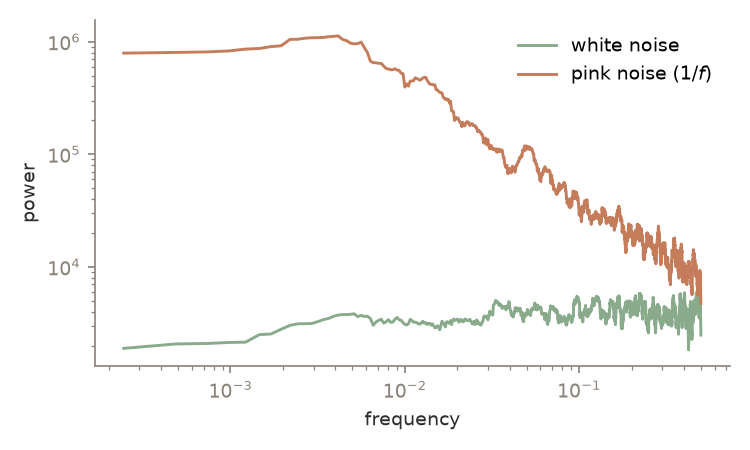
\includegraphics[width=0.7\linewidth]{notes/assets/example-psd.png}
  \caption{白噪声与粉噪声的功率谱密度（双对数坐标）。}\label{fig:psd}
\end{figure}

\subsection{子图}
用 \texttt{subfigure} 环境把多张图并排放在同一个编号下，子图自动编为 (a)、(b)，引用时显示为 \ref{fig:white}、\ref{fig:pink}：
\begin{figure}[htbp]
  \centering
  \begin{subfigure}[b]{0.4\linewidth}
    
\includegraphics[width=\linewidth]{notes/assets/example-white-noise.png}
    \caption{白噪声}\label{fig:white}
  \end{subfigure}
  \hfill
  \begin{subfigure}[b]{0.4\linewidth}
    
\includegraphics[width=\linewidth]{notes/assets/example-pink-noise.png}
    \caption{粉噪声}\label{fig:pink}
  \end{subfigure}
  \caption{两种噪声的二维样本。粉噪声（图~\ref{fig:pink}）比白噪声（图~\ref{fig:white}）具有更多低频结构。}\label{fig:noise}
\end{figure}

\subsection{并排的独立图}
两个带 \verb|\caption| 的 \texttt{minipage} 会各自编号，如图~\ref{fig:left} 与图~\ref{fig:right}：
\begin{figure}[htbp]
  \centering
  \begin{minipage}{0.4\linewidth}
    \centering
    
\includegraphics[width=\linewidth]{notes/assets/example-white-noise.png}
    \caption{独立编号的左图}\label{fig:left}
  \end{minipage}
  \hfill
  \begin{minipage}{0.4\linewidth}
    \centering
    
\includegraphics[width=\linewidth]{notes/assets/example-pink-noise.png}
    \caption{独立编号的右图}\label{fig:right}
  \end{minipage}
\end{figure}

\section{代码}\label{sec:code}
\begin{lstlisting}[language=python]
def q_sample(x0, t, noise):
    # 前向加噪，对应式 (2)
    return sqrt_ab[t] * x0 + sqrt_1m_ab[t] * noise
\end{lstlisting}

\section{引用}\label{sec:cite}
单篇引用写作 \verb|\cite{key}|~\cite{wang2020cnn}，多篇写作 \verb|\cite{a,b}|~\cite{ojha2023towards,tan2024rethinking}。
文献列表写在 \texttt{thebibliography} 环境中，编号按 \verb|\bibitem| 出现的顺序生成。
交叉引用同样适用于章节、定理和子图：表格在第~\ref{sec:table} 节，插图在第~\ref{sec:figure} 节；\verb|\autoref| 会自动带上类型名，例如 \autoref{thm:converge} 与 \autoref{fig:pink}。

\begin{quote}
用 \LaTeX{} 写博客，表格终于不再难看。
\end{quote}

\begin{thebibliography}{9}
  \bibitem{wang2020cnn} S.-Y. Wang, O. Wang, R. Zhang, A. Owens, A. A. Efros. CNN-generated images are surprisingly easy to spot\ldots\ for now. In \emph{CVPR}, 2020.
  \bibitem{ojha2023towards} U. Ojha, Y. Li, Y. J. Lee. Towards universal fake image detectors that generalize across generative models. In \emph{CVPR}, 2023.
  \bibitem{wang2023dire} Z. Wang, J. Bao, W. Zhou, W. Wang, H. Hu, H. Chen, H. Li. DIRE for diffusion-generated image detection. In \emph{ICCV}, 2023.
  \bibitem{tan2024rethinking} C. Tan, Y. Zhao, S. Wei, G. Gu, P. Liu, Y. Wei. Rethinking the up-sampling operations in CNN-based generative network for generalizable deepfake detection. In \emph{CVPR}, 2024.
\end{thebibliography}
